%% wp5 布局代数：拼接、合并、复合（论文第 3 节前半）
\wph{布局代数（Layout Algebra）}
\label{sec:layoutalgebra}

尽管 \CuTe 布局只是所有可能函数空间中的一个子集，与 {\tt BLAS}、{\tt torch.tensor} 和 {\tt numpy.ndarray} 等库中传统的扁平形状（flat-shape）与扁平步幅（flat-stride）表示相比，它们能够表示严格更大的一组布局函数。

除表示能力之外，\CuTe 布局的一项关键效用在于它们可以被操作与组合以构造新的布局。这通过对布局定义的一组核心代数运算来实现，这些运算还可进一步用于构造更高层的运算。

在本节中，我们定义{\em 布局同态}（layout homomorphism）——即接收一个或多个 \CuTe 布局、并产生一个满足某些函数性质的 \CuTe 布局的运算。

\wpsh{拼接（Concatenate）}
\label{sec:concatenation}

一个布局可以表示为其各子布局的\emph{拼接}（concatenation），
\begin{align*}
\v{L} &= S : D\\
&= (S_0, S_1, \ldots, S_n) : (D_0, D_1, \ldots, D_n) \\
&= (S_0 : D_0, S_1 : D_1, \ldots, S_n : D_n) \\
&= (\v{L}_0, \v{L}_1, \ldots, \v{L}_n)
\end{align*}
使得
\begin{align}
\forall c = (c_0,c_1,\ldots,c_n) \in \Z(\v{L}), \ \ \v{L}(c) = \v{L}_0(c_0) + \v{L}_1(c_1) + \cdots + \v{L}_n(c_n).
\label{eqn:concat}
\end{align}
要使拼接可行，函数性质~\eqref{eqn:concat} 蕴含所有子布局的陪域必须包含在同一个整数半模（integer-semimodule）之中。例如，任意两个具有整数步幅的布局都可以拼接，但布局 $4:2$ 与 $3:e_0$ 无法拼接。

注意到布局的每个子布局本身也是布局，于是可以观察到：任何操作布局的代数运算也同样可以应用到任意单个子布局上。我们常称这类运算为“逐模运算（by-mode operation）”，本节定义的每一个运算（合并、复合、补、逻辑切分等）都可以逐模应用。这一方式用如下组合子（combinator）表达：
\begin{align}
\v{A} \star  \langle \v{B}, \v{C} \rangle = (\v{A}_0, \v{A}_1) \star  \langle \v{B}, \v{C} \rangle = (\v{A}_0 \star  \v{B}, \v{A}_1 \star  \v{C}),
\label{eqn:layout_combinator}
\end{align}
其中 $\star$ 是某个作用于两个布局的运算，$\langle \rangle$ 记号表示由布局组成的元组，以区别于布局的拼接。

\wpsh{合并（Coalesce）}
\label{sec:coalesce}

给定布局 $\v{A}$，其\emph{合并}（coalesced）布局 $\v{R}$ 是满足如下性质的布局：
\begin{align}
\text{一致的整型定义域：} && \abs{\v{R}} &= \abs{\v{A}}, \\
\text{展平或整型的形状：} && \text{depth}(\v{R}) &\leq 1, \\
\text{一致的整型求值：} && \forall \bar{c} \in \Z_{\abs{\v{A}}}, \ \ \v{R}(\bar{c}) &= \v{A}(\bar{c}).
\end{align}

\texttt{coalesce} 运算通过把布局 $\v{A}$ 视作整数上的函数来“简化”它，并可能将其形状塌缩为更浅的表示。尽管这一过程可能丢失阶与层次信息、改变坐标集合、并合并 $\v{A}$ 的多个模，它保证布局作为整型坐标上的映射保持函数等价。

实践中，当提到合并布局时，我们通常指的是达到最小阶的那个合并布局。

例如，$(2,(1,6)):(1,(6,2))$ 的合并布局是 $12:1$。或者，也可以利用式~\eqref{eqn:layout_combinator} 对该布局逐模合并，即对每个模独立地应用 \texttt{coalesce}：
\begin{align*}
\texttt{coalesce}((2,(1,6)):(1,(6,2)), \ \langle \ast,\ast \rangle) &= \texttt{coalesce}((2:1,(1,6):(6,2)), \ \langle \ast,\ast \rangle) \\
&= (\texttt{coalesce}(2:1, \ \ast), \ \texttt{coalesce}((1,6):(6,2), \ \ast)) \\
&= (\texttt{coalesce}(2:1), \ \texttt{coalesce}((1,6):(6,2))) \\
&= (2:1,6:2) \\
&= (2,6):(1,2).
\end{align*}
类似地，2 阶布局 $((4,3),5):((15,1),3)$ 合并为 $(4,15):(15,1)$，而其逐模合并布局仍是 $((4,3),5):((15,1),3)$，因为行布局与列布局各自单独合并时保持不变。2 阶布局 $(4,(3,5)):(15,(1,3))$ 同样合并为 $(4,15):(15,1)$，而其逐模合并布局是 $(4,15):(15,1)$，因为第二个模可以单独合并为 $15:1$。

\wpsh{复合（Composition）}
\label{sec:composition}

给定布局 $\v{A}$ 与 $\v{B}$，\emph{群复合}（group composition）布局 $\v{R} = \v{A} \circ \v{B}$ 满足：
\begin{align}
\label{eqn:compose_compat}
\text{定义域相容性：} && \v{B} &\preceq \v{R}, \\
\label{eqn:compose_result}
\text{函数复合性：} && \forall c \in \Z(\v{B}), \ \ \v{R}(c) &= \v{A}(\v{B}(c)).
\end{align}

在这一定式中，$\v{B}$ 通过定义 $\v{R}$ 的定义域来决定结果布局的形状与坐标集合，而 $\v{A}$ 决定 $\v{R}$ 的陪域。相容性条件保证 $\v{B}$ 的{\em 所有}坐标也都可用作 $\v{R}$ 的坐标。要使群复合与函数复合均可接纳，$\v{B}$ 的陪域必须与 $\v{A}$ 的定义域相容，这通常意味着 $\v{B}$ 的陪域是一组与 $\Z(\v{A})$ 中某个坐标集合同余的坐标。

\wpssh{复合的性质（Composition Properties）}

\paragraph{恒等布局（Identity Layout）。}
对任意形状 $S$，\emph{恒等布局}（identity layout）$\v{I}_S$ 满足
\begin{align*}
\forall c \in \Z_S, \ \ \v{I}_S(c) = c.
\end{align*}
注意，只要 $S \preceq P$，$\v{I}_S$ 实际上可以取任意形状 $P$。例如，下面都是恒等布局 $\v{I}_{24}$，且对所有 $i \in \Z_{24}$ 满足 $\v{L}(i) = i$：
\begin{align*}
24 : 1, \quad (4,6) : (1,4), \quad (3,(4,2)) : (1,(3,12)).
\end{align*}
类似地，下面两者都是恒等布局 $\v{I}_{(4,6)}$，且对所有 $(i,j) \in \Z_{(4,6)}$ 满足 $\v{L}(i,j) = (i,j)$：
\begin{align*}
(4,6) : (e_0,e_1), \quad (4,(3,2)) : (e_0,(e_1,3e_1)).
\end{align*}
对陪域为 $\Z_D$ 的布局 $\v{B}$，任意 $\v{I}_D$ 都充当\emph{群复合的左单位元}（left identity），
\begin{align*}
\v{I}_D \circ \v{B} = \v{B}.
\end{align*}
对定义域为 $\Z_S$ 的布局 $\v{A}$，形状为 $S$ 的布局 $\v{I}_S$ 充当\emph{群复合的右单位元}（right identity），
\begin{align*}
\v{A} \circ \v{I}_S = \v{A}.
\end{align*}

\paragraph{结合律（Associative Property）。}
给定布局 $\v{A}$、$\v{B}$ 与 $\v{C}$，以及条件
\begin{align}
\text{image}(\v{C}) \subseteq \Z(\v{B}) \quad \text{且} \quad \text{image}(\v{B}) \subseteq \Z(\v{A}),
\label{eqn:layout_image}
\end{align}
则
\begin{align*}
\v{A} \circ (\v{B} \circ \v{C}) = (\v{A} \circ \v{B}) \circ \v{C}.
\end{align*}
注意，当式~\eqref{eqn:layout_image} 不满足时，复合往往仍然可行，但结合律可能失效。例如，
\begin{align*}
(5,3):(1,7) \ \circ \ [4:1 \ \circ \ 2:5] &&= (5,3):(1,7) \ \circ \ 2:5 &&= 2:7 \\
[(5,3):(1,7) \ \circ \ 4:1] \ \circ \ 2:5 &&= 4:1 \ \circ \ 2:5 &&= 2:5
\end{align*}
会给出不同结果，因为 $2:5$ 的值域未包含在 $4:1$ 的定义域之中。不过，鉴于 {\tt idx2crd} 与 {\tt inner\_product} 的越界行为，两个表达式都能正确求值。

\wpssh{求值与限制（Evaluation and Restrictions）}
\label{sec:composition_impl}

群复合的求值可以由式~\eqref{eqn:idx2crd} 与式~\eqref{eqn:innerprod} 中的布局求值运算构造性地推导出来。在本节中，我们确定布局 $\v{A}$ 与 $\v{B}$ 上的一组可接纳性条件，它们是成功计算群复合所必需的。

首先，我们要求 $\v{A}$ 与 $\v{B}$ 之间的函数相容性：$\v{B}$ 的陪域必须与 $\v{A}$ 的形状弱同余。最常见的情况是 $\v{B}$ 的陪域为整数，而由于所有布局 $\v{A}$ 都接受整型坐标，因此二者函数相容。更一般地，当 $\v{B}$ 产生坐标时，这些坐标必须与 $\Z(\v{A})$ 中的某个坐标同余。

一般做法是令 $(\v{A} \circ \v{B})(i)$ 与 $\v{R}(i)$ 的求值相等。实践中我们发现，只需分析取最简形式 $\v{B} = s : d$ 的基础情形，并把其他求值归约到该情形即可。

\paragraph{基础情形（Base Case）。}

设 $\v{B} = s : d$，其中 $s \in \Z^+$、$d \in \N$。设 $\v{A} = S:D = (S_0, S_1, \ldots, S_R):(D_0, D_1, \ldots, D_R)$ 为一个布局，其中 $S_r \in \Z^+$、$D_r \in \mathcal{D}$。定义 $S = (S_0, S_1, \ldots, S_R)$ 的独占前缀乘积（exclusive prefix-product）为
\begin{align*}
\bar{S}_r = \prod_{k=0}^{r-1} S_k.
\end{align*}
于是，复合 $\v{R} = \v{A} \circ \v{B}$ 对每个 $i = 0, 1, \ldots, s-1$ 的求值如下：
\begin{align}
\v{R}(i) = (\v{A} \circ \v{B})(i) &= (D \circ S \circ d \circ s)(i) \nonumber \\
&= D(S(d(s(i)))) \nonumber\\
&= \texttt{inner\_product}(\texttt{idx2crd}_S(\texttt{inner\_product}(\texttt{idx2crd}_s(i), d)), D) \nonumber \\
&= \texttt{inner\_product}(\texttt{idx2crd}_S(\texttt{inner\_product}(i, d)), D) \nonumber \\
&= \texttt{inner\_product}(\texttt{idx2crd}_S(i \cdot d), D) \nonumber \\
&= \sum_{r=0}^{R-1} \left(\floor{\frac{i \cdot d}{\bar{S}_r}} \bmod S_r\right) \cdot D_r + \floor{\frac{i \cdot d}{\bar{S}_R}} \cdot D_R
\label{eqn:ABi} \\
&= \sum_{r=0}^{R-1} \left(\floor{\frac{i}{\bar{S}'_r}} \bmod S'_r\right) \cdot D'_r + \floor{\frac{i}{\bar{S}'_R}} \cdot D'_R. \nonumber
\end{align}
结果 $\v{R}$（若存在）定义为布局 $\v{R} = S':D' = (S'_0, S'_1, \ldots, S'_R):(D'_0, D'_1, \ldots, D'_R)$。我们的目标是确定 $S'$、$D'$ 以及它们存在的条件。

首先，由于 $\v{B}$ 的陪域是整数，我们可以假设布局 $\v{A}$ 已经合并。根据定义，这不会改变复合的求值。

其次，注意到若 $(s-1) \cdot d < \bar{S}_r$，则对所有 $i < s$ 与 $q > r$ 都有 $\floor{i \cdot d / \bar{S}_q} = 0$。也就是说，$\v{A}$ 的所有满足 $q > r$ 的模对结果没有贡献。不失一般性，我们在 $(s-1) \cdot d \geq \bar{S}_R$ 的假设下继续推导；这总可以通过对 $\v{A}$ 的形状做截断或延拓来实现。该假设不会改变式~\eqref{eqn:ABi}，却通过剔除冗余情形简化了分析。

我们施加{\bf 步幅整除性条件}（stride divisibility condition）
\begin{align}
\bar{S}_r \mid d \ \text{ 或 } \ d \mid \bar{S}_r \ \text{ 对每个 } r = 0, \ldots, R,
\label{eqn:divis_stride}
\end{align}
并定义
\begin{align*}
\delta_r = \ceil{\frac{d}{\bar{S}_r}}, \quad \rho_r = \ceil{\frac{\bar{S}_r}{d}}.
\end{align*}
于是，
\begin{align*}
\sum_{r=0}^{R-1} \left(\floor{\frac{i \cdot d}{\bar{S}_r}} \bmod S_r\right) \cdot D_r + \floor{\frac{i \cdot d}{\bar{S}_R}} \cdot D_R &=
\sum_{r=0}^{R-1} \left(\floor{i \cdot \frac{\delta_r}{\rho_r}} \bmod S_r\right) \cdot D_r + \floor{i \cdot \frac{\delta_R}{\rho_R}} \cdot D_R.
\end{align*}
利用恒等式 $(a b) \bmod (n b) = (a \bmod n) \cdot b$，并注意到 $\delta_r \mid S_r$，可得：
\begin{align*}
&= \sum_{r=0}^{R-1} \left(\floor{i \cdot \frac{1}{\rho_r}} \bmod \frac{S_r}{\delta_r}\right) \cdot (D_r \cdot \delta_r) + \floor{i \cdot \frac{1}{\rho_R}} \cdot (D_R \cdot \delta_R).
\end{align*}
一旦验证了
\begin{align*}
\rho_r = \ceil{\frac{\bar{S}_r}{d}} = \ceil{\frac{\prod_{k=0}^{r-1} S_k}{d}} = \ceil{\frac{S_0}{d}} \ceil{\frac{\prod_{k=1}^{r-1} S_k}{\ceil{d / S_0}}} = \cdots = \prod_{k=0}^{r-1} \ceil{\frac{S_k}{\ceil{d / \bar{S}_k}}} = \prod_{k=0}^{r-1} \ceil{\frac{S_k}{\delta_k}} = \bar{S}'_r,
%\rho_0 = 1 = \bar{S}'_0 \\
%\rho_1 = \ceil{\frac{S_0}{d}} = \ceil{\frac{S_0}{\delta_0}} = \bar{S}'_1 \\
%\rho_2 = \ceil{\frac{S_0S_1}{d}} = \ceil{\frac{S_0}{d}\frac{S_1}{d}} = \ceil{\frac{S_0}{d}}\ceil{\frac{S_1}{\ceil{d / S_0}}} = \ceil{\frac{S_0}{\delta_0}}\ceil{\frac{S_1}{\delta_1}} = \bar{S}'_2
\end{align*}
结果的形状与步幅即可辨识为
\begin{align*}
S'_r &= \frac{S_r}{\delta_r}, \\
D'_r &= D_r \cdot \delta_r.
\end{align*}

为满足相容性条件~\eqref{eqn:compose_compat}，形状还必须满足 $\abs{S'} = \bar{S}'_{R+1} = s$。为此，我们再施加{\bf 形状整除性条件}（shape divisibility condition）：
\begin{align}
\ceil{\frac{\bar{S}_r}{d}} \mid s \ \text{ 对每个 } r = 0, \ldots, R,
\label{eqn:divis_shape}
\end{align}
并将形状修改为
\begin{align*}
S'_r &= \frac{S_r}{\delta_r}, \quad S'_R = \frac{s}{\rho_R}, \\
D'_r &= D_r \cdot \delta_r,
\end{align*}
其中项 $s / \rho_R$ 用于将结果形状截断或延拓到大小 $s$。

这样，只要 $\v{A}$ 与 $\v{B}$ 满足步幅整除性条件~\eqref{eqn:divis_stride} 与形状整除性条件~\eqref{eqn:divis_shape}，我们就求出了结果 $\v{R} = S':D'$ 的形状与步幅。

\paragraph{归约情形：分配律（Reductive Case: Distributive）。}

为了用基础情形表达更一般的复合，我们利用复合运算对 $\v{B}$ 的子布局拼接的分配性质，
\begin{align}
\v{A} \circ \v{B} &= \v{A} \circ (\v{B}_0, \v{B}_1, \ldots) = (\v{A} \circ \v{B}_0, \v{A} \circ \v{B}_1, \ldots).
\label{eqn:layout_distributivity}
\end{align}
当 $\v{A}$ 的形状 $S$ 对 $\v{B}$ 的各子布局之和可分配时，该性质成立，
\begin{align}
%\forall c = (c_0, c_1, \ldots) \in \Z_{\v{B}}, \\
(\v{A} \circ \v{B})(c)
%= (D \circ S \circ \v{B})(c)
&= D(S(\v{B}(c))) \notag \\
&= D(S(\v{B}_0(c_0) + \v{B}_1(c_1) + \cdots)) && \text{$\v{B} = (\v{B}_0, \v{B}_1, \ldots)$ 的拼接} \notag \\
&\stackrel{?}{=} D(S(\v{B}_0(c_0)) + S(\v{B}_1(c_1)) + \cdots) && \text{以 $S$ 对 $\v{B}_i$ 的分配性为条件} \label{eqn:shape_distributivity} \\
&= D(S(\v{B}_0(c_0))) + D(S(\v{B}_1(c_1))) + \cdots && \text{$D$ 的线性性} \notag \\
%&= (\v{A} \circ \v{B}_0)(c_0) + (\v{A} \circ \v{B}_1)(c_1) + \cdots \notag \\
&= (\v{A} \circ \v{B}_0, \v{A} \circ \v{B}_1,\ldots)(c) \notag
\end{align}
以下两个条件之一即足以满足式~\eqref{eqn:shape_distributivity}：
\begin{compactitem}
\item $\v{B}$ 的陪域与形状 $S$ 同余。此时 $S$ 的作用是恒等变换，显然可分配。
\item 当 $S$ 不是恒等变换时，则必须有
\begin{align*}
\floor{\frac{\sum_i c_i \cdot d_i}{\bar{S}_r}} \bmod S_r &= \sum_i \floor{\frac{c_i \cdot d_i}{\bar{S}_r}} \bmod S_r \ \ \text{ 对每个 } r = 0, \ldots, R-1 \text{ 成立，且 } \\
\floor{\frac{\sum_i c_i \cdot d_i}{\bar{S}_R}} &= \sum_i \floor{\frac{c_i \cdot d_i}{\bar{S}_R}}
\end{align*}
而这发生在如下情形：
\begin{enumerate}[itemsep=0pt,topsep=2pt]
\item 所有基础子布局的步幅 $d_i$ 都满足步幅整除性条件~\eqref{eqn:divis_stride}，且
\item 所有基础子布局 $s_i : d_i$ 的像集彼此分离，
\begin{align*}
\forall i,j, \ \ s_i \cdot d_i \leq d_j \ \ \text{ 或 } \ \ s_j \cdot d_j \leq d_i
\end{align*}
\end{enumerate}
\end{compactitem}

\paragraph{归约情形：坐标（Reductive Case: Coordinate）。}

当 $\v{B}$ 产生坐标时，这些坐标必须与 $\Z(\v{A})$ 中的某个坐标同余，且 $\v{B}$ 的每个步幅都必须是某个坐标整数半模的缩放基元素：$d = a \cdot e_i \in \Z^{S'}$，其中 $S' \preceq \v{A}$。当这些条件满足时，我们观察到
\begin{align*}
\v{A} \circ \v{B} = \v{A} \circ (a \cdot e_i) \circ s = \v{A}_i \circ a \circ s = \v{A}_i \circ \v{B}',
\end{align*}
这就回到了基础情形，其中 $\v{B}' = s : a$ 是一个陪域为整数的 1 阶、深度为 0 的布局。对于具有其他整数半模步幅的 $\v{B}$，必须特别小心地将 $\v{B}$ 的陪域映射到 $\v{A}$ 的定义域，并且可能需要对 $\v{A}$ 与 $\v{B}$ 施加额外的限制。

\wpssh{直观理解与整除性（Intuition and Divisibility）}

与 1 阶左操作数布局 $\v{A}$ 的复合是平凡的，因为 $S_R$ 不会出现在式~\eqref{eqn:ABi} 中：
\begin{align*}
(S_0):(D_0) \ \circ \  s:d = s:D_0 \cdot d.
\end{align*}
此时不存在非平凡的整除性检查，因为 $R = 0$、$\bar{S}_0 = 1$、$\delta_0 = d$ 且 $\rho_0 = 1$。注意，这意味着即使 $\text{image}(\v{B}) \not\subseteq \Z(\v{A})$，群复合依然可行，
\begin{align*}
7:11 \ \circ \ 3:4 = 3:44,
\end{align*}
而且 $\v{B}$ 无须两两不相交即可满足分配性，
\begin{align*}
7:11 \ \circ \ (3,5):(6,3) = (3,5):(66,33).
\end{align*}

对于与更高阶布局 $\v{A}$ 的复合，直观策略包含两步：
\begin{compactitem}
\item 通过从 $\v{A}$ 中“切分掉”（divide out）前 $d$ 个元素，确定一个产生 $\v{A}$ 的每第 $d$ 个元素的中间布局。
\item 通过“保留”（keep）前 $s$ 个元素，把该中间带步幅布局的大小固定为 $s$。
\end{compactitem}
例如，
\begin{align*}
(4,6,8,10):(2,3,5,7) \ \circ \  6:12
\end{align*}
等价于
\begin{align*}
(4,6,8,10):(2,3,5,7) \ \circ \  6:12 = (1,2,8,10):(X,9,5,7) \ \circ \  6:1,
\end{align*}
其中 $\v{A}$ 的前 12 个元素被“切分掉”，步幅相应地缩放。然后，修改后布局的前 6 个元素被“保留”，得到：
\begin{align*}
(1,2,8,10):(X,9,5,7) \ \circ \  6:1 = (2,3):(9,5).
\end{align*}
或者，我们也可以先“保留”前 $6 \cdot 12$ 个元素，再“切分掉”前 12 个，如下所示：
\begin{align*}
(4,6,8,10):(2,3,5,7) \ \circ \  6:12 = (4,6,3):(2,3,5) \ \circ \  6:12 = (2,3):(9,5).
\end{align*}
整除性条件保证“切分掉”与“保留”两步中的逐次除法对结果形状总是产生整数。

\paragraph{对整除性条件的违反（Violations of Divisibility Conditions）。}
某些复合会违反步幅或形状整除性条件。例如，
\begin{align*}
(4,6,8):(2,3,5) \ \circ \  6:3
\end{align*}
违反了步幅整除性条件~\eqref{eqn:divis_stride}，因为 $\bar{S}_1 = 4$ 与 $d = 3$ 不可整除。不存在能表示布局 $(4,6,8):(2,3,5)$ 的每第 3 个元素的布局。

类似地，复合
\begin{align*}
(4,6,8):(2,3,5) \ \circ \  6:1
\end{align*}
违反了形状整除性条件~\eqref{eqn:divis_shape}，因为 $\left\lceil \frac{\bar{S}_1}{d} \right\rceil = \left\lceil \frac{4}{1} \right\rceil = 4$ 不能整除 $s = 6$。不存在能表示 $(4,6,8):(2,3,5)$ 的前 6 个元素的布局。

归根结底，这意味着 \CuTe 布局在群复合下并非严格封闭。然而在实践中，违反整除性条件往往源于概念性的应用错误、布局与硬件不相容、程序员失误等问题。这些错误大多可以在编译期被捕获，从而有助于提升程序安全性与开发效率。

\paragraph{表面上的违反（Apparent Violations）。}

考虑复合
\begin{align*}
(4,2,8):(3,12,97) \ \circ \  3:3,
\end{align*}
它看似违反了步幅整除性条件，因为 $\bar{S}_1 = 4$ 与 $d = 3$ 不可整除。这一问题可以通过对 $\v{A}$ 做合并（如第~\ref{sec:composition_impl} 节所述）以及对 $\v{A}$ 做截断（正如 $(s-1) \cdot d < \bar{S}_r$ 情形中所处理的那样）来解决。等价的复合产生结果
\begin{align*}
(4,2,8):(3,12,97) \ \circ \  3:3 = (8,8):(3,97) \ \circ \  3:3 = (8):(3) \ \circ \  3:3 = 3:9.
\end{align*}
然而，下面的复合不满足整除性条件：
\begin{align*}
(4,2,8):(3,12,97) \ \circ \  4:3 && (4,2,8):(3,15,97) \ \circ \  3:3.
\end{align*}
左侧的例子无法被充分截断，而右侧的例子则无法被合并。


\wpssh{应用：划分示例（Application: Partitioning Example）}
\label{sec:layouttv}

复合位于 \CuTe 布局代数的核心，支撑着重塑形（reshaping）、重定步幅（restriding）、置换（permuting）、划分（partitioning）、分块（tiling）以及提取子布局等运算。本节演示如何利用复合、以任意的线程-值模式（thread-value pattern）对一个数据张量进行划分。

\begin{figure}[ht]
\centering
\scalebox{0.6}{
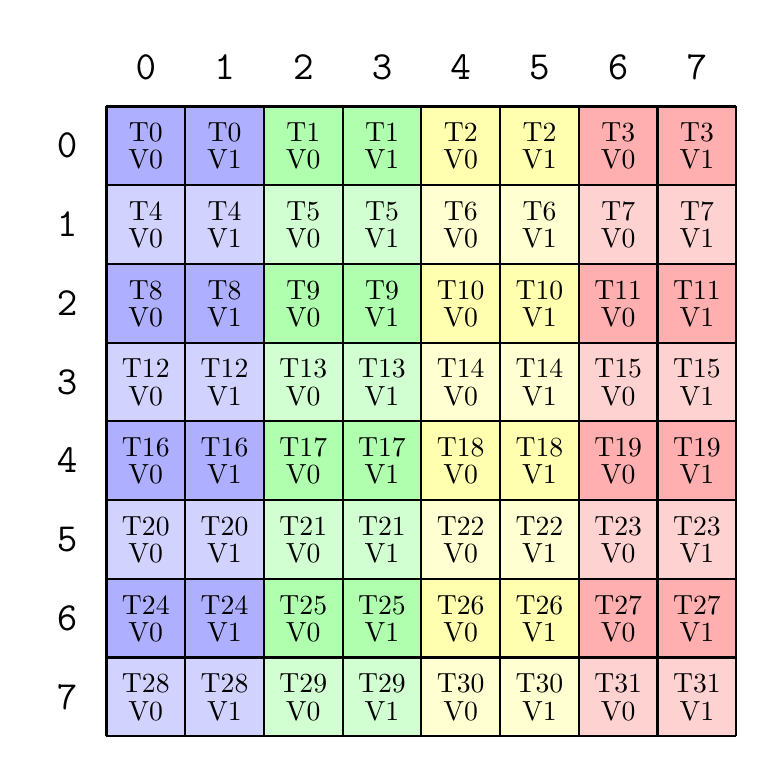
\begin{tikzpicture}[x={(0cm,-1cm)},y={(1cm,0cm)},every node/.style={minimum size=1cm, outer sep=0pt}]
\node[fill={rgb,255:red,175;green,175;blue,255}] at (0,0) {\shortstack{T0 \\ V0}};
\node[fill={rgb,255:red,175;green,175;blue,255}] at (0,1) {\shortstack{T0 \\ V1}};
\node[fill={rgb,255:red,175;green,255;blue,175}] at (0,2) {\shortstack{T1 \\ V0}};
\node[fill={rgb,255:red,175;green,255;blue,175}] at (0,3) {\shortstack{T1 \\ V1}};
\node[fill={rgb,255:red,255;green,255;blue,175}] at (0,4) {\shortstack{T2 \\ V0}};
\node[fill={rgb,255:red,255;green,255;blue,175}] at (0,5) {\shortstack{T2 \\ V1}};
\node[fill={rgb,255:red,255;green,175;blue,175}] at (0,6) {\shortstack{T3 \\ V0}};
\node[fill={rgb,255:red,255;green,175;blue,175}] at (0,7) {\shortstack{T3 \\ V1}};
\node[fill={rgb,255:red,210;green,210;blue,255}] at (1,0) {\shortstack{T4 \\ V0}};
\node[fill={rgb,255:red,210;green,210;blue,255}] at (1,1) {\shortstack{T4 \\ V1}};
\node[fill={rgb,255:red,210;green,255;blue,210}] at (1,2) {\shortstack{T5 \\ V0}};
\node[fill={rgb,255:red,210;green,255;blue,210}] at (1,3) {\shortstack{T5 \\ V1}};
\node[fill={rgb,255:red,255;green,255;blue,210}] at (1,4) {\shortstack{T6 \\ V0}};
\node[fill={rgb,255:red,255;green,255;blue,210}] at (1,5) {\shortstack{T6 \\ V1}};
\node[fill={rgb,255:red,255;green,210;blue,210}] at (1,6) {\shortstack{T7 \\ V0}};
\node[fill={rgb,255:red,255;green,210;blue,210}] at (1,7) {\shortstack{T7 \\ V1}};
\node[fill={rgb,255:red,175;green,175;blue,255}] at (2,0) {\shortstack{T8 \\ V0}};
\node[fill={rgb,255:red,175;green,175;blue,255}] at (2,1) {\shortstack{T8 \\ V1}};
\node[fill={rgb,255:red,175;green,255;blue,175}] at (2,2) {\shortstack{T9 \\ V0}};
\node[fill={rgb,255:red,175;green,255;blue,175}] at (2,3) {\shortstack{T9 \\ V1}};
\node[fill={rgb,255:red,255;green,255;blue,175}] at (2,4) {\shortstack{T10 \\ V0}};
\node[fill={rgb,255:red,255;green,255;blue,175}] at (2,5) {\shortstack{T10 \\ V1}};
\node[fill={rgb,255:red,255;green,175;blue,175}] at (2,6) {\shortstack{T11 \\ V0}};
\node[fill={rgb,255:red,255;green,175;blue,175}] at (2,7) {\shortstack{T11 \\ V1}};
\node[fill={rgb,255:red,210;green,210;blue,255}] at (3,0) {\shortstack{T12 \\ V0}};
\node[fill={rgb,255:red,210;green,210;blue,255}] at (3,1) {\shortstack{T12 \\ V1}};
\node[fill={rgb,255:red,210;green,255;blue,210}] at (3,2) {\shortstack{T13 \\ V0}};
\node[fill={rgb,255:red,210;green,255;blue,210}] at (3,3) {\shortstack{T13 \\ V1}};
\node[fill={rgb,255:red,255;green,255;blue,210}] at (3,4) {\shortstack{T14 \\ V0}};
\node[fill={rgb,255:red,255;green,255;blue,210}] at (3,5) {\shortstack{T14 \\ V1}};
\node[fill={rgb,255:red,255;green,210;blue,210}] at (3,6) {\shortstack{T15 \\ V0}};
\node[fill={rgb,255:red,255;green,210;blue,210}] at (3,7) {\shortstack{T15 \\ V1}};
\node[fill={rgb,255:red,175;green,175;blue,255}] at (4,0) {\shortstack{T16 \\ V0}};
\node[fill={rgb,255:red,175;green,175;blue,255}] at (4,1) {\shortstack{T16 \\ V1}};
\node[fill={rgb,255:red,175;green,255;blue,175}] at (4,2) {\shortstack{T17 \\ V0}};
\node[fill={rgb,255:red,175;green,255;blue,175}] at (4,3) {\shortstack{T17 \\ V1}};
\node[fill={rgb,255:red,255;green,255;blue,175}] at (4,4) {\shortstack{T18 \\ V0}};
\node[fill={rgb,255:red,255;green,255;blue,175}] at (4,5) {\shortstack{T18 \\ V1}};
\node[fill={rgb,255:red,255;green,175;blue,175}] at (4,6) {\shortstack{T19 \\ V0}};
\node[fill={rgb,255:red,255;green,175;blue,175}] at (4,7) {\shortstack{T19 \\ V1}};
\node[fill={rgb,255:red,210;green,210;blue,255}] at (5,0) {\shortstack{T20 \\ V0}};
\node[fill={rgb,255:red,210;green,210;blue,255}] at (5,1) {\shortstack{T20 \\ V1}};
\node[fill={rgb,255:red,210;green,255;blue,210}] at (5,2) {\shortstack{T21 \\ V0}};
\node[fill={rgb,255:red,210;green,255;blue,210}] at (5,3) {\shortstack{T21 \\ V1}};
\node[fill={rgb,255:red,255;green,255;blue,210}] at (5,4) {\shortstack{T22 \\ V0}};
\node[fill={rgb,255:red,255;green,255;blue,210}] at (5,5) {\shortstack{T22 \\ V1}};
\node[fill={rgb,255:red,255;green,210;blue,210}] at (5,6) {\shortstack{T23 \\ V0}};
\node[fill={rgb,255:red,255;green,210;blue,210}] at (5,7) {\shortstack{T23 \\ V1}};
\node[fill={rgb,255:red,175;green,175;blue,255}] at (6,0) {\shortstack{T24 \\ V0}};
\node[fill={rgb,255:red,175;green,175;blue,255}] at (6,1) {\shortstack{T24 \\ V1}};
\node[fill={rgb,255:red,175;green,255;blue,175}] at (6,2) {\shortstack{T25 \\ V0}};
\node[fill={rgb,255:red,175;green,255;blue,175}] at (6,3) {\shortstack{T25 \\ V1}};
\node[fill={rgb,255:red,255;green,255;blue,175}] at (6,4) {\shortstack{T26 \\ V0}};
\node[fill={rgb,255:red,255;green,255;blue,175}] at (6,5) {\shortstack{T26 \\ V1}};
\node[fill={rgb,255:red,255;green,175;blue,175}] at (6,6) {\shortstack{T27 \\ V0}};
\node[fill={rgb,255:red,255;green,175;blue,175}] at (6,7) {\shortstack{T27 \\ V1}};
\node[fill={rgb,255:red,210;green,210;blue,255}] at (7,0) {\shortstack{T28 \\ V0}};
\node[fill={rgb,255:red,210;green,210;blue,255}] at (7,1) {\shortstack{T28 \\ V1}};
\node[fill={rgb,255:red,210;green,255;blue,210}] at (7,2) {\shortstack{T29 \\ V0}};
\node[fill={rgb,255:red,210;green,255;blue,210}] at (7,3) {\shortstack{T29 \\ V1}};
\node[fill={rgb,255:red,255;green,255;blue,210}] at (7,4) {\shortstack{T30 \\ V0}};
\node[fill={rgb,255:red,255;green,255;blue,210}] at (7,5) {\shortstack{T30 \\ V1}};
\node[fill={rgb,255:red,255;green,210;blue,210}] at (7,6) {\shortstack{T31 \\ V0}};
\node[fill={rgb,255:red,255;green,210;blue,210}] at (7,7) {\shortstack{T31 \\ V1}};
\draw[color=black,thick,shift={(-0.5,-0.5)}] (0,0) grid (8,8);
\node at (0,-1) {\Large{\texttt{0}}};
\node at (1,-1) {\Large{\texttt{1}}};
\node at (2,-1) {\Large{\texttt{2}}};
\node at (3,-1) {\Large{\texttt{3}}};
\node at (4,-1) {\Large{\texttt{4}}};
\node at (5,-1) {\Large{\texttt{5}}};
\node at (6,-1) {\Large{\texttt{6}}};
\node at (7,-1) {\Large{\texttt{7}}};
\node at (-1,0) {\Large{\texttt{0}}};
\node at (-1,1) {\Large{\texttt{1}}};
\node at (-1,2) {\Large{\texttt{2}}};
\node at (-1,3) {\Large{\texttt{3}}};
\node at (-1,4) {\Large{\texttt{4}}};
\node at (-1,5) {\Large{\texttt{5}}};
\node at (-1,6) {\Large{\texttt{6}}};
\node at (-1,7) {\Large{\texttt{7}}};
\end{tikzpicture}
}
\caption{Ampere FP64 Tensor Core 所要求的 $8 {\times} 8$ C 矩阵的线程-值划分。}
\label{fig:TVLayout}
\end{figure}

考察一个细化了形状 $(8,8)$ 的数据布局。我们的目标是使用图~\ref{fig:TVLayout} 所示的线程-值模式对该数据进行划分，该模式是某个特定 Ampere Tensor Core 的逻辑划分模式。这条指令的线程-值划分模式可以用布局
\begin{align*}
\texttt{ThrValLayoutC:} \quad ((4,8),2):((16,1),8),
\end{align*}
表示，它充当从 $(\texttt{thread\_idx}, \texttt{value\_idx})$ 到 $8 {\times} 8$ 矩阵内一维坐标的映射。如图所示，出于人类可读性的考虑，图~\ref{fig:TVLayout} 实际上画出的是其逆——它展示的是从 $8 {\times} 8$ 矩阵内的二维坐标到 $(\texttt{thread\_idx}, \texttt{value\_idx})$ 二元组的映射。这个 {\tt ThrValLayoutC} 被视为 Ampere Tensor Core 指令的静态元数据——它是指令与硬件功能的内在属性；在 \CuTe 出现之前，它只能以指令集架构（ISA）中类似图~\ref{fig:TVLayout} 的图像来描述。

任意 $8 {\times} 8$ 数据布局都可以通过与线程-值布局 {\tt ThrValLayoutC} 复合而被置换。每次复合都会产生一个与形状 $(32,2)$ 相容的布局，并定义 $(\texttt{thread\_idx}, \texttt{value\_idx})$ 与数据偏移之间的映射。例如，表~\ref{tab:TVLayoutExamples} 展示了若干数据布局经上述 {\tt ThrValLayoutC} 复合变换的例子。

\begin{table}[ht]
\centering
\begin{tabular}{|c|c|c|c|}
数据名称 & 数据布局 $8 {\times} 8$（$\v{A}$） & 线程-值布局 $32 {\times} 2$（$\v{B}$） & 结果 $32 {\times} 2$（$\v{R}$） \\ \hline \hline
{\tt ColMajor} & $(8,8):(1,8)$ & $((4,8),2):((16,1),8)$ & $((4,8),2):((16,1),8)$ \\ \hline
{\tt RowMajor} & $(8,8):(8,1)$ & $((4,8),2):((16,1),8)$ & $((4,8),2):((2,8),1)$ \\ \hline
{\tt Padded} & $(8,8):(1,9)$ & $((4,8),2):((16,1),8)$ & $((4,8),2):((18,1),9)$ \\ \hline
{\tt ColInterleaved} & $((4,2),(2,4)):((2,16),(1,8))$ & $((4,8),2):((16,1),8)$ & $((4,(4,2)),2):((8,(2,16)),1)$ \\ \hline
{\tt Swizzled} & $(8,8):(f_1,f_9)$ & $((4,8),2):((16,1),8)$ & $((4,8),2):((f_{18},f_1),f_9)$ \\ \hline
{\tt Coordinate} & $(8,8):(e_0,e_1)$ & $((4,8),2):((16,1),8)$ & $((4,8),2):((2e_1,e_0),e_1)$ \\ \hline
\end{tabular}
\caption{数据布局经线程-值（TV）布局复合变换的示例。}
\label{tab:TVLayoutExamples}
\end{table}

下面的代码展示了一种使用线程-值划分的常见模式：
\begin{python}
smem_data = Tensor(MyAccessor, MyLayout8x8)     # Tensor：Coord -> Offset
tv_layout   = Layout(((4,8),2), ((16,1),8))     # TV 布局：(Thr,Val) -> Coord
smem_tv     = composition(smem_data, tv_layout) # 复合：(Thr,Val) -> Offset
smem_v      = smem_tv[thr_id, None]             # 按线程切片得到子张量
copy(smem_v, rmem_data)                         # 拷贝到寄存器张量/数组
\end{python}
这一模式在 SIMD 编程中极为常见：每个处理元素接收某个父数据的一个对称划分。一般而言，\CuTe 认识到任意划分都可以定义为复合（置换和/或重塑形）之后再切片。如第~\ref{sec:slicing} 节所述，这种“复合-切片”模式把划分模式（{\tt ThrValLayoutC}）与实际切出的数据切片（以 {\tt thr\_id} 做的切片）分离开来。由于划分模式往往是指令或优化参数相关的编译期元数据，而切片往往是运行时的程序标识索引，这一模式更有能力传播静态信息并降低运行时开销。

\wpssh{逐模复合与分块器（By-mode Composition and Tilers）}
\label{sec:tiler}

群复合可以逐模应用，从而支持对布局的子定义域进行操作。例如，常常需要对矩阵的行与列独立地应用复合。我们使用式~\eqref{eqn:layout_combinator} 中的组合子，并把其中的 $\star$ 运算取为群复合 $\circ$，从而对布局的各个独立子布局分别应用复合。

我们把式~\eqref{eqn:layout_combinator} 中的布局元组称为{\em 分块器}（Tiler）。
\begin{definition}
{\em 分块器}（Tiler）是一个 $\texttt{HTuple}(\texttt{Tile})$，其中每个 \texttt{Tile} 是
\begin{compactitem}
\item 一个 \textit{Layout} $S:D$，或
\item 一个 \textit{Integer} $S$，等价地视作布局 $S:1$。
\end{compactitem}
\end{definition}
该定义意味着所有布局都是分块器，所有整数也都是分块器，并且允许 $(4,8)$ 这样的形状用作分块器。图~\ref{fig:48tile} 展示了这一常见情形：形状可以作为提取并操作子布局的便捷分块器。

\begin{figure}[ht]
\centering
\begin{subfigure}{0.22\textwidth}
\centering
\resizebox{\linewidth}{!}{
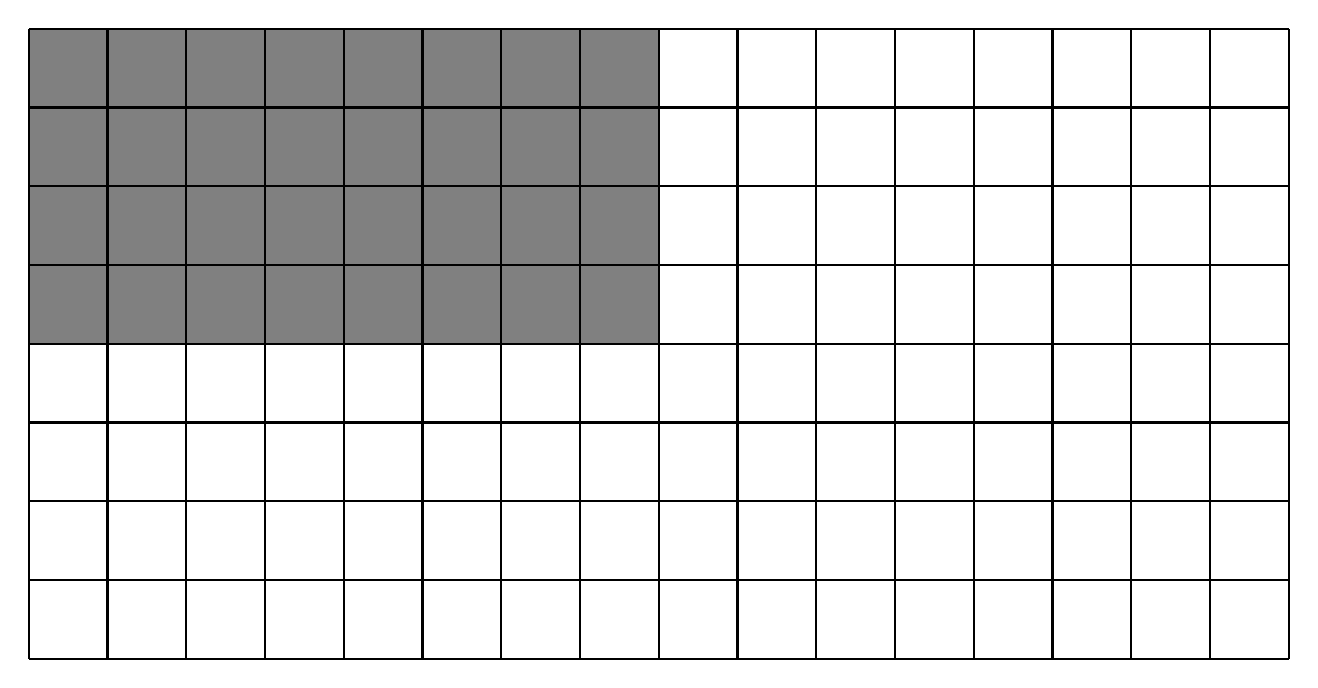
\begin{tikzpicture}[x={(0cm,-1cm)},y={(1cm,0cm)},every node/.style={minimum size=1cm, outer sep=0pt}]
\foreach \i in {0,1,2,3} {
\foreach \j in {0,1,2,3,4,5,6,7} {
\node[fill=gray] at (\i,\j) {};
}}
\draw[color=black,thick,shift={(-0.5,-0.5)}] (0,0) grid (8,16);
\end{tikzpicture}}
\caption{$\langle 4:1,8:1 \rangle \equiv \langle 4,8 \rangle$}
\label{fig:48tile}
\end{subfigure}\quad
\begin{subfigure}{0.22\textwidth}
\centering
\resizebox{\linewidth}{!}{
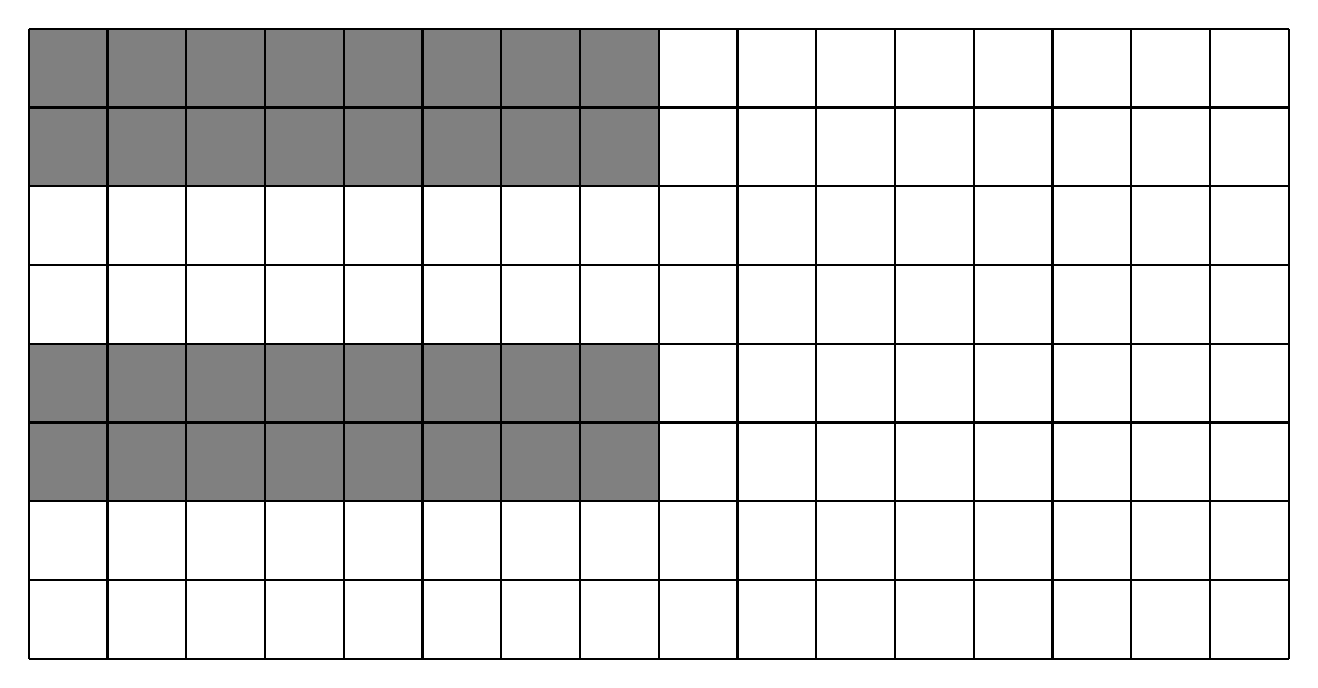
\begin{tikzpicture}[x={(0cm,-1cm)},y={(1cm,0cm)},every node/.style={minimum size=1cm, outer sep=0pt}]
\foreach \i in {0,1,4,5} {
\foreach \j in {0,1,2,3,4,5,6,7} {
\node[fill=gray] at (\i,\j) {};
}}
\draw[color=black,thick,shift={(-0.5,-0.5)}] (0,0) grid (8,16);
\end{tikzpicture}}
\caption{$\langle (2,2):(1,4),8:1 \rangle$}
\end{subfigure}\quad
\begin{subfigure}{0.22\textwidth}
\centering
\resizebox{\linewidth}{!}{
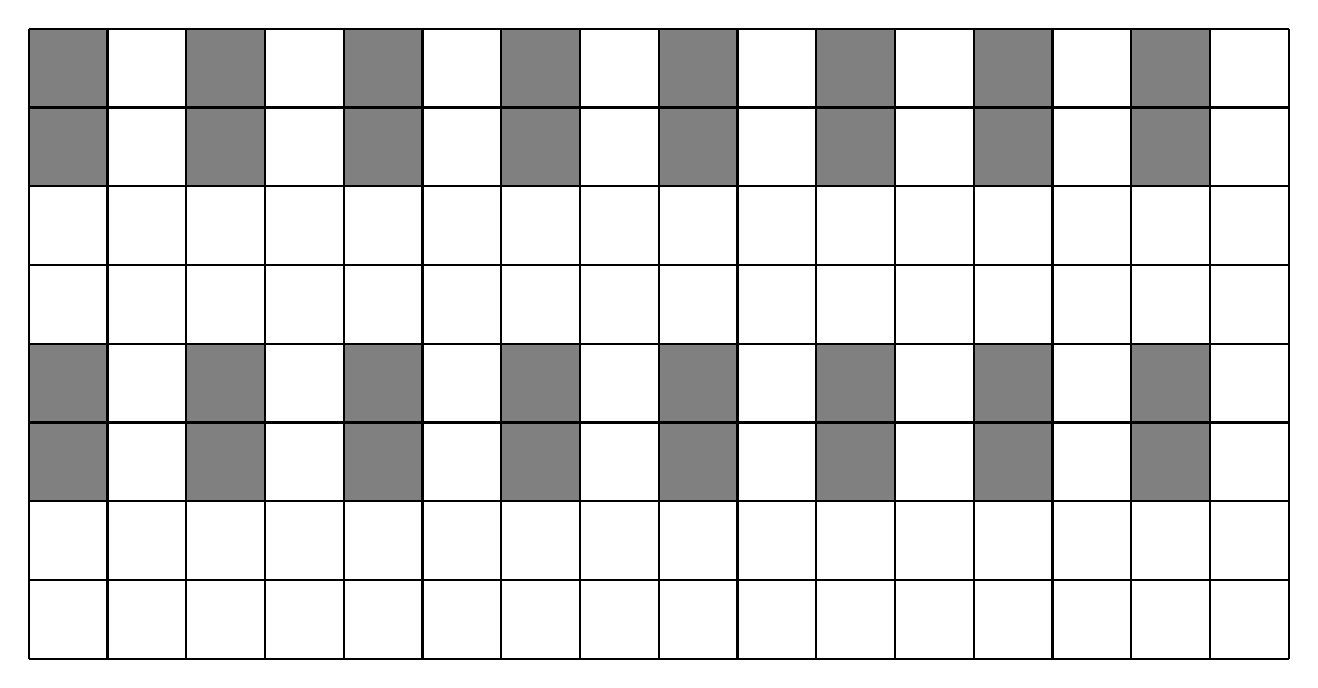
\begin{tikzpicture}[x={(0cm,-1cm)},y={(1cm,0cm)},every node/.style={minimum size=1cm, outer sep=0pt}]
\foreach \i in {0,1,4,5} {
\foreach \j in {0,2,4,6,8,10,12,14} {
\node[fill=gray] at (\i,\j) {};
}}
\draw[color=black,thick,shift={(-0.5,-0.5)}] (0,0) grid (8,16);
\end{tikzpicture}}
\caption{$\langle (2,2):(1,4),8:2 \rangle$}
\end{subfigure}\quad
\begin{subfigure}{0.22\textwidth}
\centering
\resizebox{\linewidth}{!}{
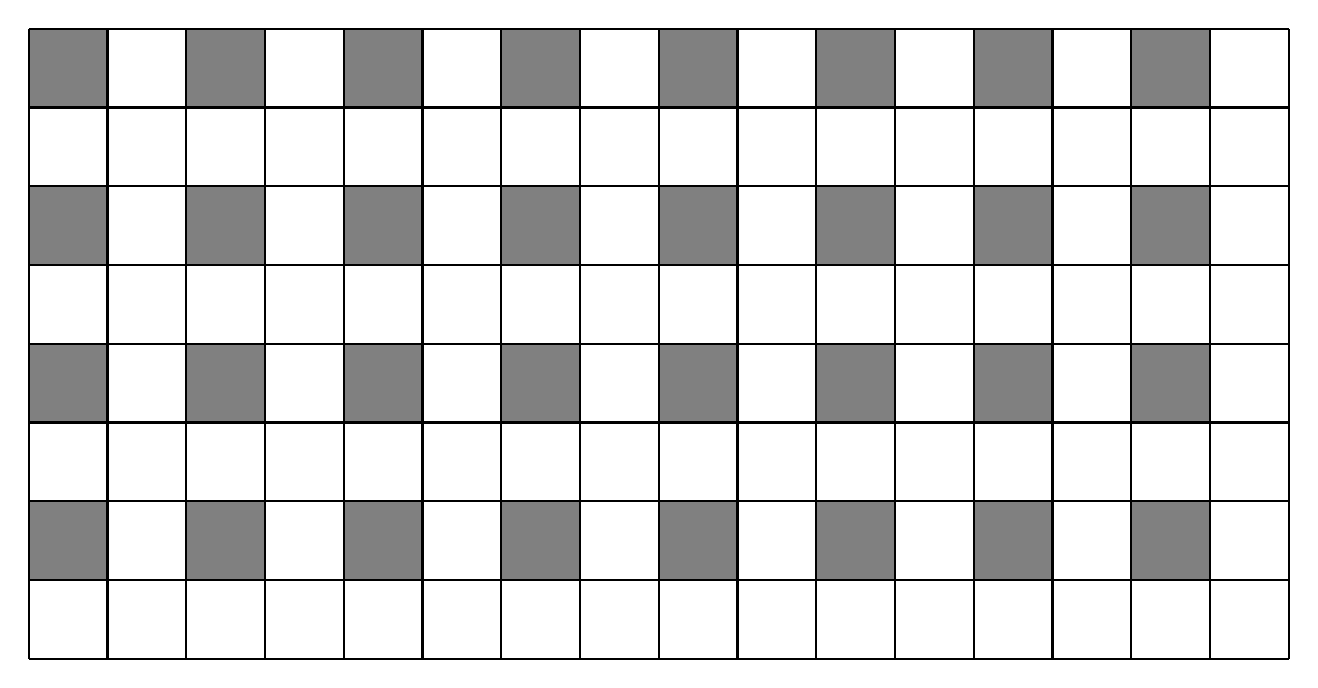
\begin{tikzpicture}[x={(0cm,-1cm)},y={(1cm,0cm)},every node/.style={minimum size=1cm, outer sep=0pt}]
\foreach \i in {0,2,4,6} {
\foreach \j in {0,2,4,6,8,10,12,14} {
\node[fill=gray] at (\i,\j) {};
}}
\draw[color=black,thick,shift={(-0.5,-0.5)}] (0,0) grid (8,16);
\end{tikzpicture}}
\caption{$\langle 4:2,8:2 \rangle$}
\end{subfigure}
\caption{通过 $\v{L} \circ \v{T}$ 从任意 $8{\times}16$ 布局 $\v{L}$ 中提取 $4 {\times} 8$ 子布局的分块器 $\v{T}$ 示例。}
\label{fig:tilers}
\end{figure}

图~\ref{fig:tilers} 展示了分块器如何通过复合作用于任意布局。图中取一个与形状 $(8,16)$ 相容的任意布局，并应用各种分块器分别从列和行中提取元素，从而产生与形状 $(4,8)$ 相容的子布局。例如，分块器 $\langle 4:1, 8:1 \rangle$ 从每列提取前 4 个元素、从每行提取前 8 个元素，产生与形状 $(4,8)$ 相容的子布局。

此外，分块器的复合与坐标布局的复合之间存在等价关系。对布局 $\v{L} = (M,N) : (X,Y)$ 与分块器 $\v{T} = \langle \v{T}_0, \v{T}_1 \rangle$，我们注意到
\begin{align*}
\v{L} \ \circ \ \v{T} \ \equiv \ \v{L} \ \circ \ (M,N):(e_0,e_1) \ \circ \ \v{T}
\end{align*}
这意味着 $(M,N):(e_0,e_1) \ \circ \ \v{T}$ 对 $\v{L}$ 的作用与 $\v{T}$ 的作用相同。这里 $(M,N):(e_0,e_1)$ 是一个恒等布局，把二维自然坐标映射到二维坐标。分块器的这种表述巩固了如下观念：形状可以被视为从坐标到自然坐标的映射，正如第~\ref{sec:layout} 节中 Layout 的定义所采用的那样。具体而言，在复合中以下对象应视为等价：
\begin{align*}
(4,8) \equiv \langle 4, 8 \rangle \equiv (4:1, 8:1) \equiv (4,8):(e_0,e_1)
\end{align*}
